\subsection{Modellbildung und Bestimmung der Systemgrößen}
Mit Hilfe der Bewegungsgleichungen aus Abschnitt \ref{Dynamik_sec} kann nun eine Zustandsraumdarstellung aufgestellt werden. Hierfür werden die nichtlinearen Terme entsprechend linearisiert. Mit Hilfe der Bewegungsgleichungen bzw. Zustandsraumdarstellung kann ein Simulink-Modell implementiert werden um das Systemverhalten zu simulieren. Mit Hilfe der Zustandsraumdarstellung wird ein Zustandsregler entworfen, welcher an dem Modell erprobt werden kann. Zusätzlich über die Simulation der Einfluss der einzelnen Parameter, Sensorrauschen und Störungen untersucht werden.

\begin{equation}
\textbf{x} = \begin{pmatrix}
\varphi \\ \dot{\varphi} \\ \dot{\psi}
\end{pmatrix}
\hspace{35pt}
\textbf{y} = \begin{pmatrix}
\varphi \\ \dot{\varphi} \\ \dot{\psi}
\end{pmatrix}
\hspace{35pt}
u = T_M
\end{equation}

\begin{equation}
\dot{\textbf{x}} = \textbf{A} \cdot \textbf{x} + \textbf{B} \cdot u
\end{equation}

\begin{equation}
\textbf{y} = \textbf{C} \cdot \textbf{x} + \textbf{D} \cdot u
\end{equation}

\begin{equation}
\begin{split}
\renewcommand*{\arraystretch}{1.7}
\textbf{A} = \begin{pmatrix}
0 & 1 & 0 \\
\frac{g(m_K \cdot l_{AC} + m_R \cdot l_{AB})}{{\theta}^A_K + m_R \cdot l_{AB}^2} &
\frac{-C_{\varphi}}{{\theta}^A_K + m_R \cdot l_{AB}^2} & 
\frac{C_{\psi}}{{\theta}^A_K + m_R \cdot l_{AB}^2} \\
\frac{-g(m_K \cdot l_{AC} + m_R \cdot l_{AB)}}{{\theta}^A_K + m_R \cdot l_{AB}^2} &
\frac{C_{\varphi}}{{\theta}^A_K + m_R \cdot l_{AB}^2} &
\frac{-C_{\psi}({\theta}^A_K + {\theta}^B_R + m_R \cdot l_{AB}^2)}{{\theta}^B_R({\theta}^A_K + m_R \cdot l_{AB}^2)}
\end{pmatrix} 
\\
\renewcommand*{\arraystretch}{1.7}
\textbf{B} = \begin{pmatrix}
0 \\ \frac{-1}{{\theta}^A_K + m_R \cdot l_{AB}^2} \\ \frac{{\theta}^A_K + {\theta}^B_R + m_R \cdot l_{AB}^2}{{\theta}^K_R({\theta}^A_K + m_R \cdot l_{AB}^2}
\end{pmatrix}
\hspace{35 pt}
\textbf{C} = \begin{pmatrix}
1 & 1 & 1
\end{pmatrix}
\hspace{35pt}
\textbf{D} = \begin{pmatrix}
0
\end{pmatrix}
\end{split}
\end{equation}

\subsubsection{Identifikation der Parameter}
Der Reglerentwurf und die Simulation erfordern eine möglichst präzise Bestimmung der Systemparameter, wie z.B. Längen, Massen, Massenträgheitsmomente und Reibwerte. Die Bestimmung der Längen $l_{AB}$ und $l_{AC}$, der Massen $m_K$, $m_R$ und $m_G$, der Massenträgheitsmomente $\theta^A_K$ und $\theta^B_R$ erfolgt über das CAD-Modell. Hierfür werden Bauteile mit einer nicht homogenen Massenverteilung, wie z.B. die Motoren, in separate Baugruppen mit homogener Massenverteilung unterteilt.

\subsubsubsection{Ermittlung des Reibwertes $C_{\varphi}$}
In dem die Schwungmasse fest mit der Würfelseite verbunden wird ergibt sich die folgende Bewegungsgleichung für das Gesamtsystem.

\begin{equation}
\label{ermittlung_c_phi_equation}
(\theta^A_K + \theta^B_R + m_R  \cdot l_{AB}^2) \ddot{\varphi} = g(m_K \cdot l_{AC} + m_R \cdot l_{AB})sin(\varphi) - C_{\varphi} \cdot \dot{\varphi}
\end{equation}

In dem Versuchsaufbau wird das Gesamtsystem nun von einem Startwinkel $\varphi_0$ losgelassen, woraufhin eine gedämpfte Schwingung entsteht. Mit Hilfe der Sensoren können die Größen $\varphi$, $\dot{\varphi}$ und $\ddot{\varphi}$ gemessen werden.

\begin{figure}[h!]
\centering
 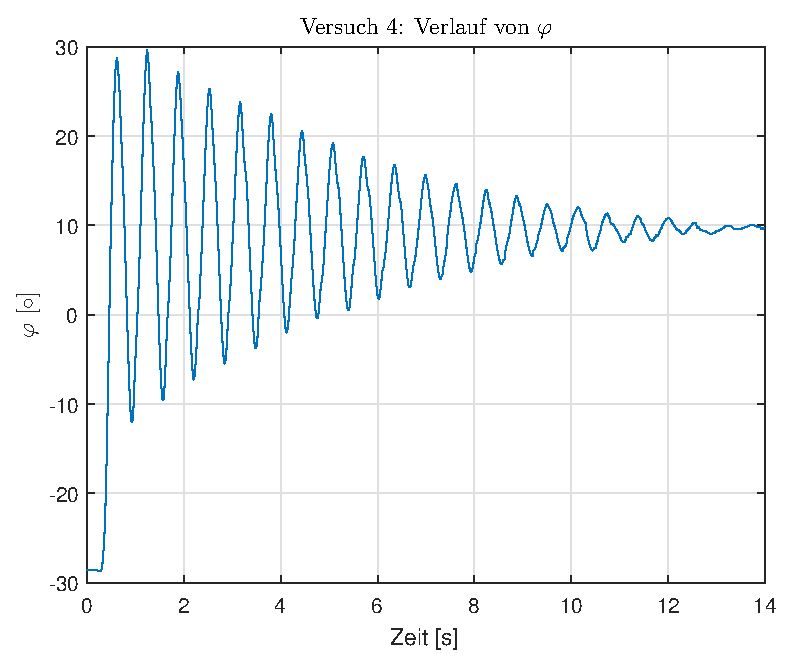
\includegraphics[width=0.5\linewidth]{img/V4_phi.eps}
	\caption{Ausfallwinkel der Würfelseite bei Versuch 4, Quelle: eigene Darstellung}
\end{figure}

Über die $n$ Messpunkte ergeben sich die folgenden Vektoren.

\begin{equation}
\boldsymbol{\varphi} = \begin{pmatrix} \varphi_1 \\ \varphi_2 \\ \vdots \\ \varphi_n \end{pmatrix} \hspace{35pt}
\boldsymbol{\dot{\varphi}} = \begin{pmatrix}
\dot{\varphi_1} \\ \dot{\varphi_2} \\ \vdots \\ \dot{\varphi_n}
\end{pmatrix} \hspace{35pt}
\boldsymbol{\ddot{\varphi}} = \begin{pmatrix}
\ddot{\varphi_1} \\ \ddot{\varphi_2} \\ \vdots \\ \ddot{\varphi_n}
\end{pmatrix}
\end{equation}

Damit ergibt sich durch Umstellen von \ref{ermittlung_c_phi_equation} die folgende Gleichung.

\begin{equation}
C_{\varphi} \cdot \boldsymbol{\dot{\varphi}} = g(m_K \cdot l_{AC} + m_R \cdot l_{AB})sin(\boldsymbol{\varphi}) - (\theta^A_K + \theta^B_R + m_R  \cdot l_{AB}^2) \boldsymbol{\ddot{\varphi}}
\end{equation}

Mit Hilfe der Methode der kleinsten Fehlerquadrate kann nun der Reibwert $C_{\varphi}$ bestimmt werden.

\begin{equation}
C_{\varphi} = 6.2 \cdot 10^{-3} \cdot kg \cdot m^2 \cdot s^{-1}
\end{equation}


\subsubsubsection{Ermittlung des Reibwertes $C_{\psi}$}
Im nächsten Versuchsaufbau wird die Würfelseite fixiert ($\dot{\varphi} = 0$). Hierbei beschleunigt der Motor die Schwungmasse mit einem konstanten Drehmoment $T_M=10mNm$. $T_M$ ist so zu wählen, dass sich die Radgeschwindigkeit $\dot{\psi}$ in einem Bereich bewegt, welcher dem Arbeitsbereich des geschlossenen Regelkreises entspricht. 

\begin{figure}[h!]
\centering
\includegraphics[width=0.5\linewidth]{img/V5_C_psi_d.eps}
\caption{Versuch 5: Verlauf der Radgeschwindigkeit, Quelle: eigene Darstellung}
\end{figure}


Da die Bewegung auf einen Freiheitsgrad beschränkt wurde vereinfacht sich das Modell des Systems auf die folgende Bewegungsgleichung.

\begin{equation}
\label{ermittlung_c_psi_equation}
\theta^B_R \cdot \ddot{\psi} = T_M - C_\psi \cdot \dot{\psi}
\end{equation}

Im Versuchsverlauf werden bei $n$ Stützstellen die Werte von $\psi$, $\dot{\psi}$ und $\ddot{\psi}$ gemessen. Daraus ergeben sich die folgenden Vektoren.

\begin{equation}
\label{ermittlung_c_psi_vektoren_equation}
\boldsymbol{\psi} = \begin{pmatrix} \psi_1 \\ \psi_2 \\ \vdots \\ \psi_n \end{pmatrix} \hspace{35pt}
\boldsymbol{\dot{\psi}} = \begin{pmatrix}
\dot{\psi_1} \\ \dot{\psi_2} \\ \vdots \\ \dot{\psi_n}
\end{pmatrix} \hspace{35pt}
\boldsymbol{\ddot{\psi}} = \begin{pmatrix}
\ddot{\psi_1} \\ \ddot{\psi_2} \\ \vdots \\ \ddot{\psi_n}
\end{pmatrix}
\end{equation}

Durch Einsetzen von \ref{ermittlung_c_psi_vektoren_equation} in \ref{ermittlung_c_psi_equation} kann über die Methode der kleinsten Fehlerquadrate wiederum der Reibwert $C_\psi$ bestimmt werden.

\begin{equation}
C_{\psi}= 3.1176 \cdot 10^{-5} \cdot kg \cdot m^2 \cdot s^{-1}
\end{equation}

\subsubsubsection{Resultate der Systemidentifikation}
An Hand der beschriebenen Versuche und Methoden wurden die folgenden Werte für die Parameter des Gesamtsystems ermittelt.

\begin{table}[h]
\centering
\begin{tabular}{|c|c|}
	\hline
	\textbf{Parameter} & \textbf{Wert} \\ \hline
	$l_{AB}$ & $0.084m$\\ \hline
	$l_{AC}$ & $0.087m$ \\ \hline
	$m_K$ & $0.221kg$ \\ \hline
	$m_R$ & $0.09kg$ \\ \hline
	${\theta}^A_K$ & $2.8 \cdot 10^{-3}kg \cdot m^2$ \\ \hline
	${\theta}^B_R$ & $1.1683 \cdot 10^{e-4} \cdot kg \cdot m^2$ \\ \hline
	$C_{\varphi}$ & $6.2 \cdot 10^{-3} \cdot kg \cdot m^2 \cdot s^{-1}$ \\ \hline
	$C_{\psi}$ & $3.1176 \cdot 10^{-5} \cdot kg \cdot m^2 \cdot s^{-1}$ \\ \hline
	$r_{S1}$ & $0.14m$ \\ \hline
	$r_{S2}$ & $0.061m$ \\ \hline
\end{tabular}
\end{table}

\newpage
\subsubsection{Entwurf des Simulink-Modelles}
Dieser Abschnitt erklärt den Aufbau des Simulink-Modelles zur Simulation des Systems. Die oberste Modellschicht besteht aus drei Subsystemen zur Simulation des Motor, der Würfelseite und der Schwungmasse.

\begin{figure}[h]
\label{Simulink_1DModell_Overview}
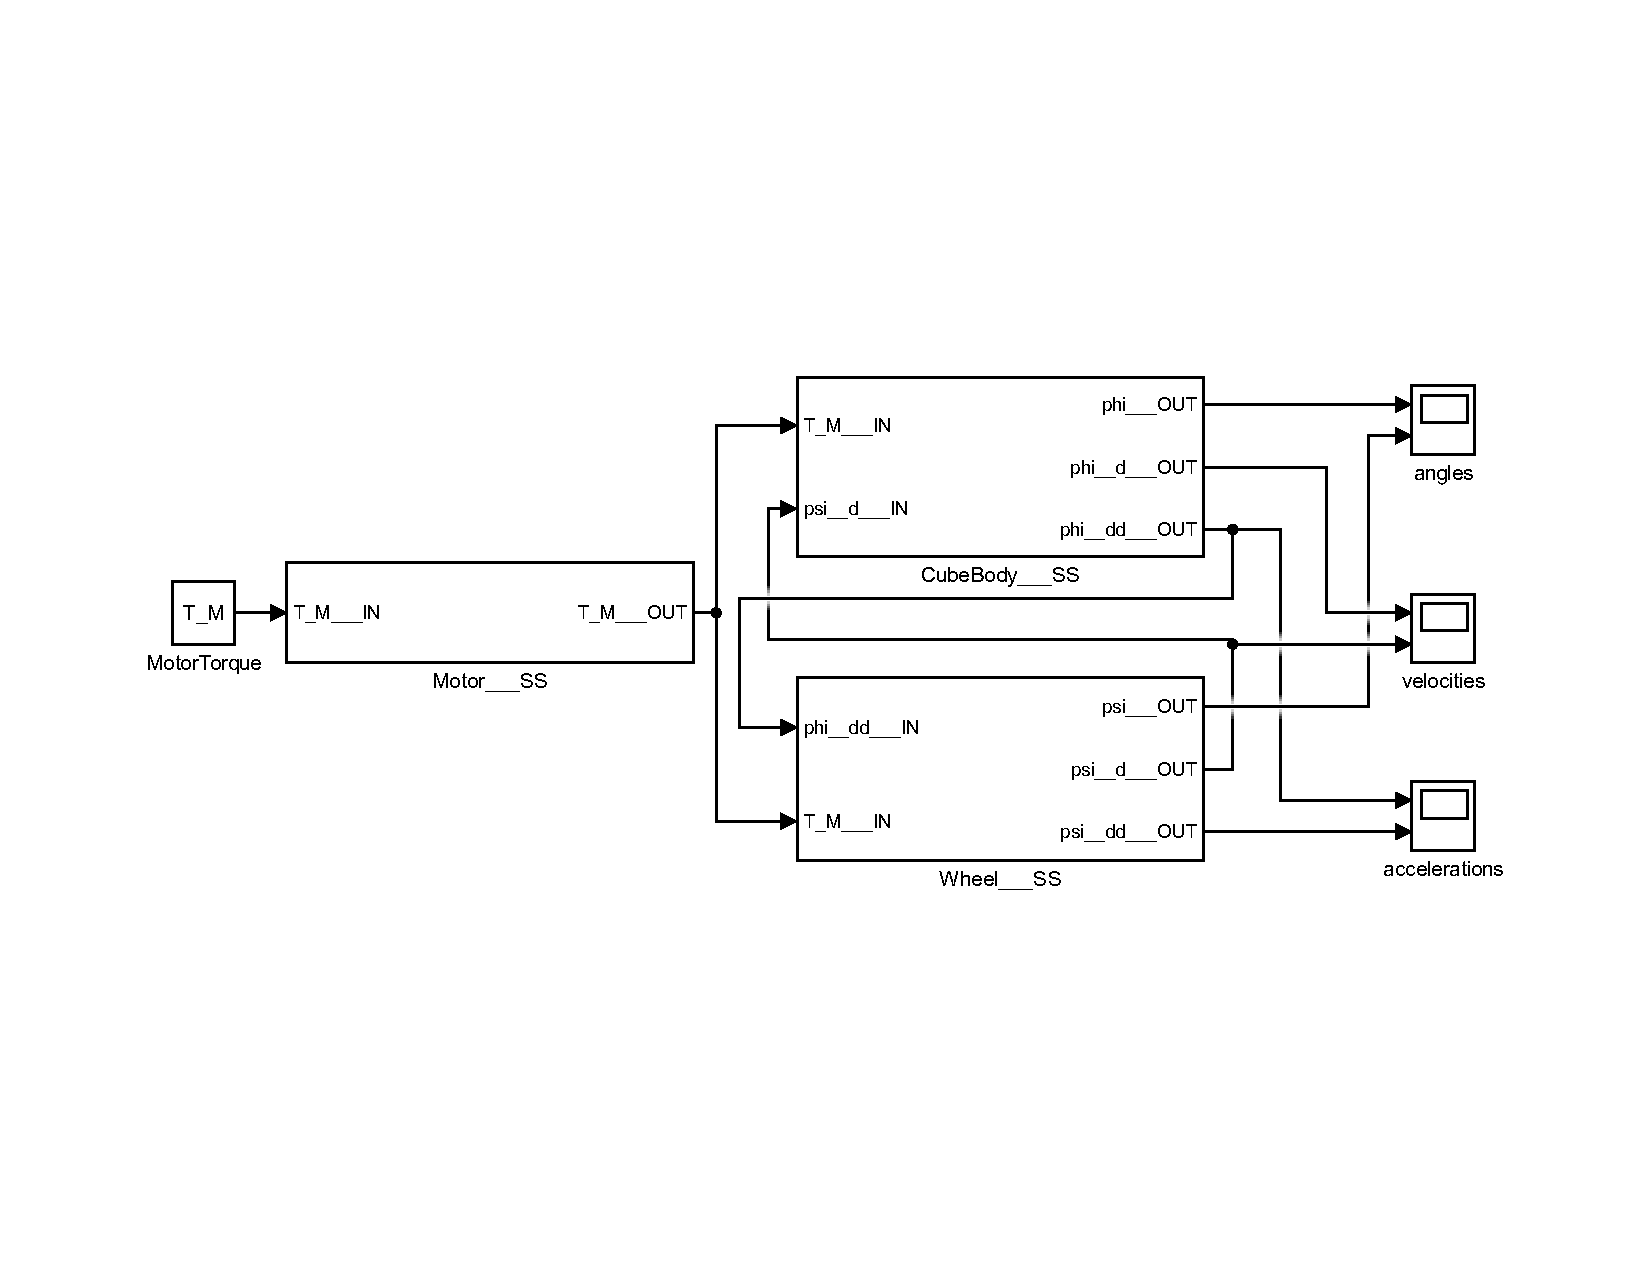
\includegraphics[width=\linewidth, trim={0 7cm 0 6cm},clip]{model_1D_overview}
\caption{Simulink-Modell Übersicht, Quelle: eigene Darstellung}
\end{figure}

\subsubsubsection{Simulation des Motors}
Der Motor wird als zwei in Reihe geschaltete PT1-Glieder simuliert. Da der Regler als Stellgröße ein Motormoment berechnet, beträgt die Verstärkung des Motor $K_M$ in der Simulation den Wert eins. Die Zeitkonstanten der PT1-Glieder sind einerseits die elektrische Zeitkonstante $T_e$ und die mechanische Zeitkonstante $T_m$, wessen Werte dem Datenblatt des Herstellers entnommen werden.

\begin{equation}
K_M = 1 \hspace{35pt} T_e = 0.55ms \hspace{35pt} T_m = 12.4ms
\end{equation}

\subsubsubsection{Simulation der Würfelseite}
Die Dynamik der Würfelseite wird von \ref{BG_phi_quation} beschrieben.

\begin{equation}
\ddot{\varphi} = \frac{g(m_R \cdot l_{AB}^2 + m_K \cdot l_{AC})sin(\varphi) - C_{\varphi} \cdot \dot{\varphi} + C_{\psi} \cdot \dot{\psi} - T_M}{{\theta}^A_K + m_R \cdot l_{AB}^2} \tag{\ref{BG_phi_quation}}
\end{equation}

Somit ist die Winkelbeschleunigung gleich der Summe der Drehmomente geteilt durch die betroffenen Massenträgheitsmomente. Durch Integration und Rückführung können die einzelnen Drehmomente berechnet werden. Das folgende Modell zeigt die Umsetzung dieser Berechnungsvorschrift in Simulink.

\begin{figure}[h]
\label{Simulink_1DModell_CubeBody_pic}
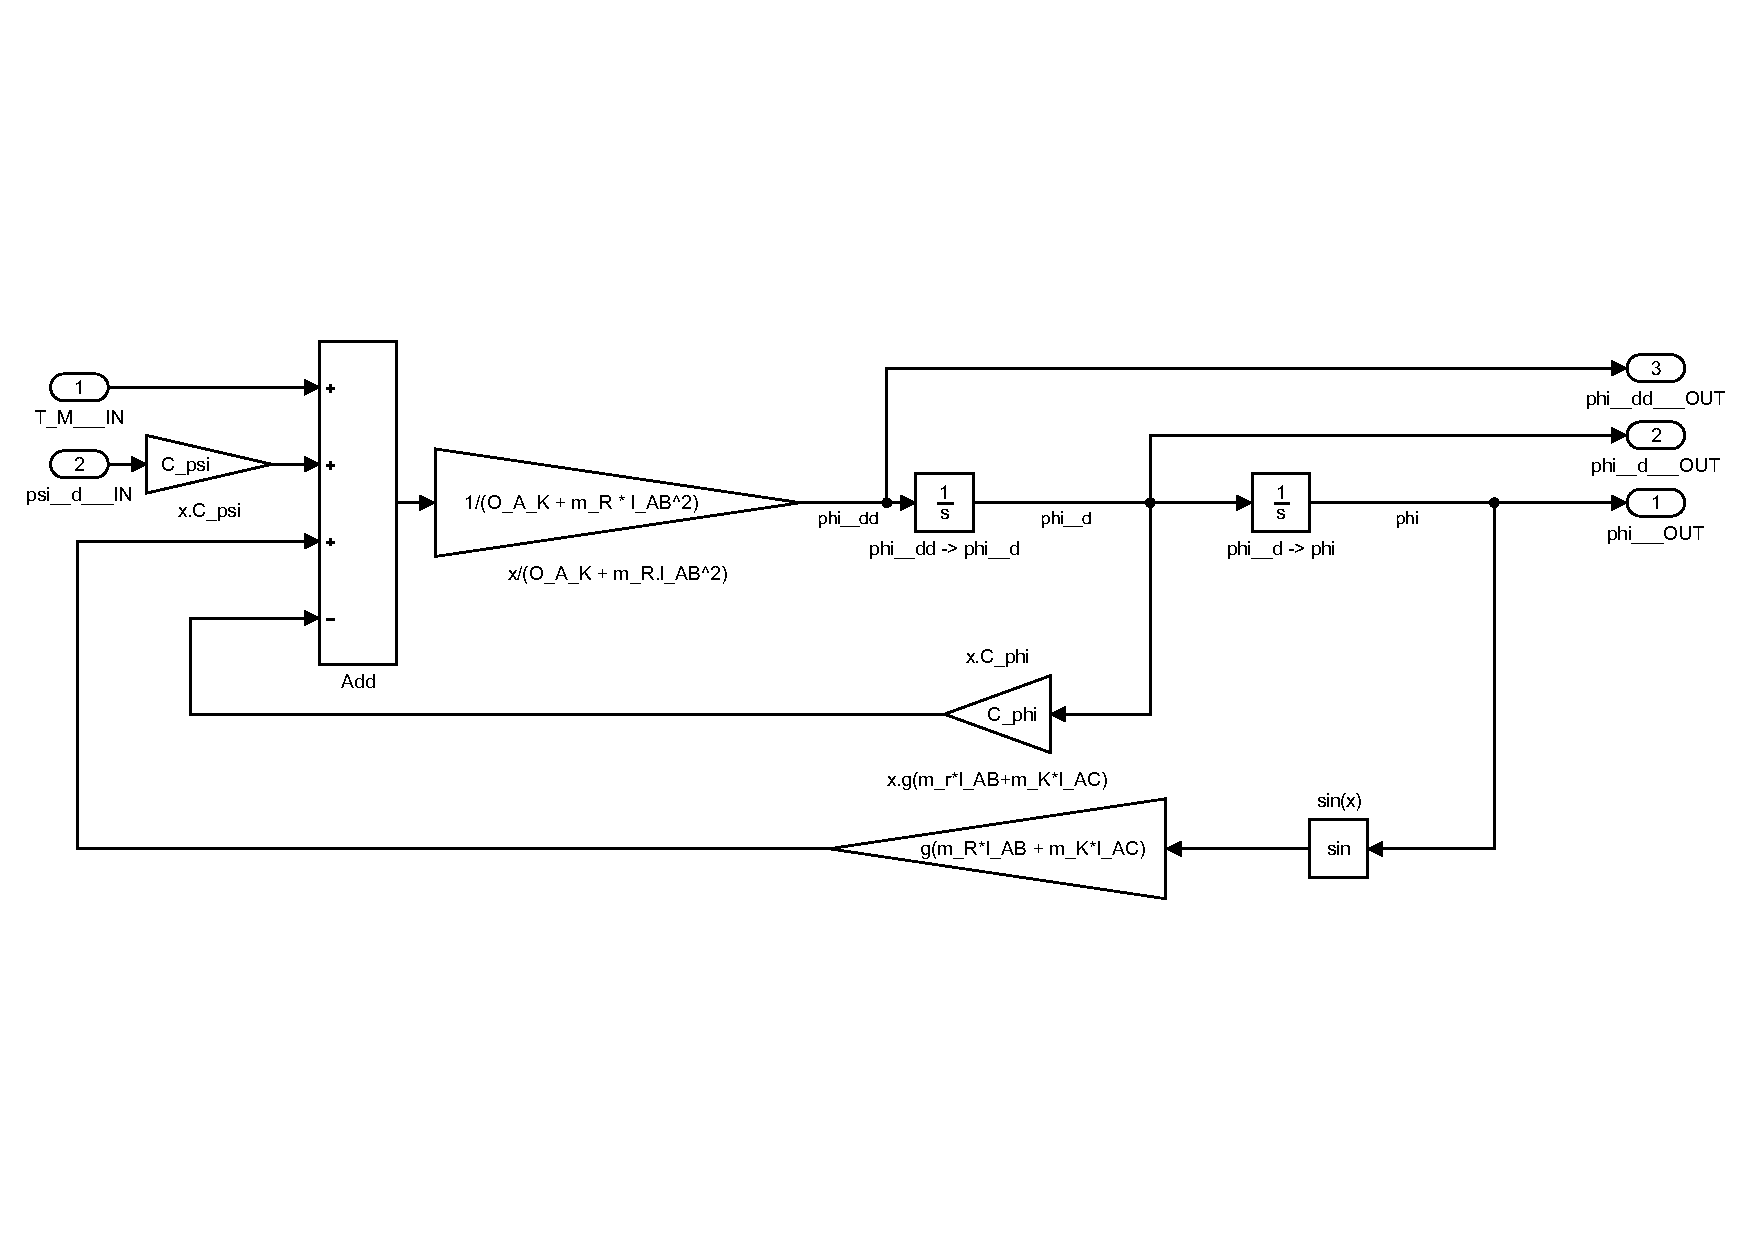
\includegraphics[width=\linewidth, trim={0 5cm 0 5cm},clip]{model_1D_cubebody}
\caption{Subsystem Würfelseite, Quelle: eigene Darstellung}
\end{figure}

\subsubsubsection{Simulation der Schwungmasse}
Die Dynamik der Schwungmasse wird von \ref{BG_psi_equation} beschrieben, allerdings wird das Modell vereinfacht indem $\ddot{phi}$ nicht substituiert wird.

\begin{equation}
{\theta}^R_B \cdot \ddot{\psi} = T_M - C_{\psi} \cdot \dot{\psi} - {\theta}^B_R \cdot \ddot{\varphi}\tag{\ref{BG_psi_equation}}
\end{equation}

Das Simulink-Modell folgt dem selben Schema wie das Subsystem zur Simulation der Bewegung des Würfelkörpers.

\begin{figure}[h]
\label{Simulink_1DModell_Wheel_pic}
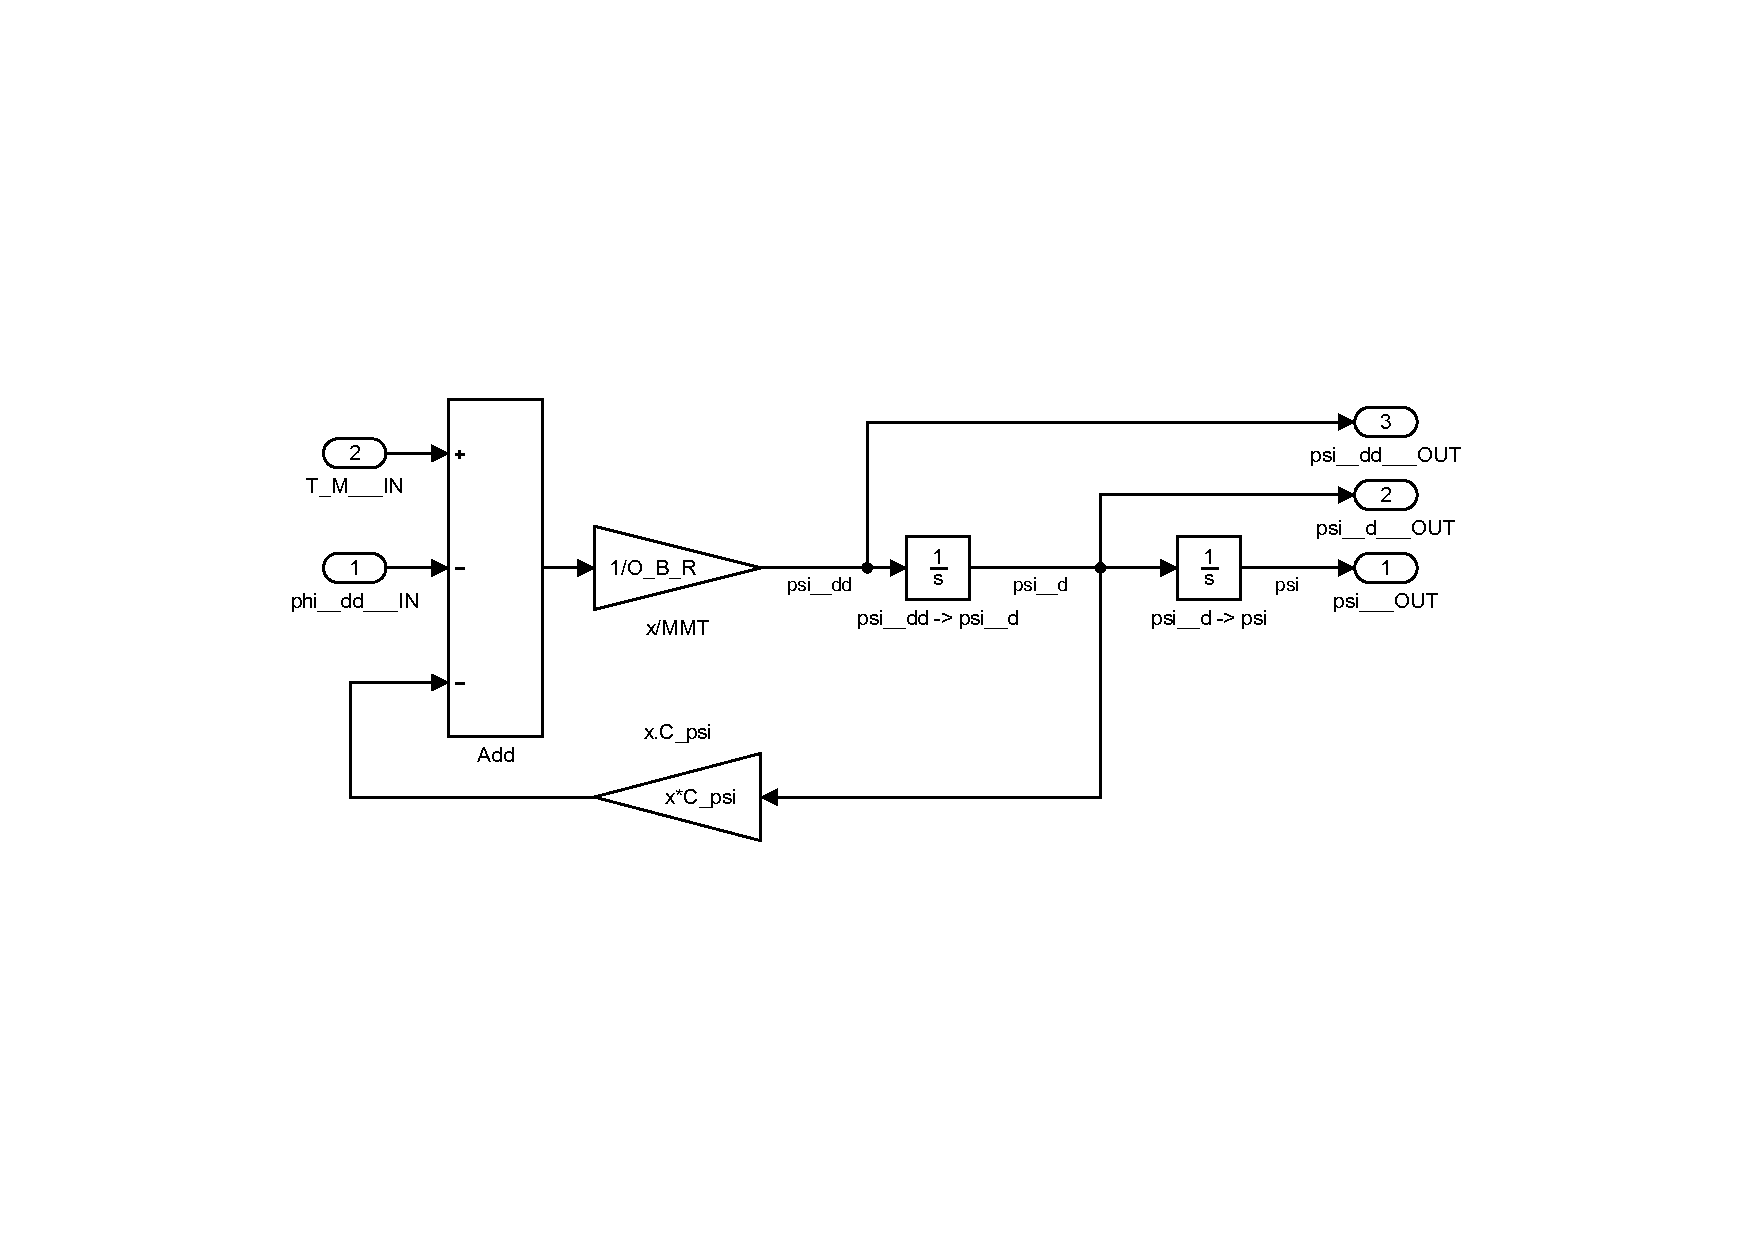
\includegraphics[width=\linewidth, trim={0 6cm 0 6cm},clip]{model_1D_wheel}
\caption{Subsystem Schwungmasse, Quelle: eigene Darstellung}
\end{figure}